% Options for packages loaded elsewhere
\PassOptionsToPackage{unicode}{hyperref}
\PassOptionsToPackage{hyphens}{url}
\PassOptionsToPackage{dvipsnames,svgnames,x11names}{xcolor}
%
\documentclass[
  english,
  a4paper,
]{article}
\usepackage{amsmath,amssymb}
\usepackage{lmodern}
\usepackage{iftex}
\ifPDFTeX
  \usepackage[T1]{fontenc}
  \usepackage[utf8]{inputenc}
  \usepackage{textcomp} % provide euro and other symbols
\else % if luatex or xetex
  \usepackage{unicode-math}
  \defaultfontfeatures{Scale=MatchLowercase}
  \defaultfontfeatures[\rmfamily]{Ligatures=TeX,Scale=1}
\fi
% Use upquote if available, for straight quotes in verbatim environments
\IfFileExists{upquote.sty}{\usepackage{upquote}}{}
\IfFileExists{microtype.sty}{% use microtype if available
  \usepackage[]{microtype}
  \UseMicrotypeSet[protrusion]{basicmath} % disable protrusion for tt fonts
}{}
\makeatletter
\@ifundefined{KOMAClassName}{% if non-KOMA class
  \IfFileExists{parskip.sty}{%
    \usepackage{parskip}
  }{% else
    \setlength{\parindent}{0pt}
    \setlength{\parskip}{6pt plus 2pt minus 1pt}}
}{% if KOMA class
  \KOMAoptions{parskip=half}}
\makeatother
\usepackage{xcolor}
\IfFileExists{xurl.sty}{\usepackage{xurl}}{} % add URL line breaks if available
\IfFileExists{bookmark.sty}{\usepackage{bookmark}}{\usepackage{hyperref}}
\hypersetup{
  pdftitle={Interaction structure constrains the emergence of conventions in group communication},
  pdflang={en},
  colorlinks=true,
  linkcolor={blue},
  filecolor={Maroon},
  citecolor={blue},
  urlcolor={blue},
  pdfcreator={LaTeX via pandoc}}
\urlstyle{same} % disable monospaced font for URLs
\usepackage[margin=25mm]{geometry}
\usepackage{longtable,booktabs,array}
\usepackage{calc} % for calculating minipage widths
% Correct order of tables after \paragraph or \subparagraph
\usepackage{etoolbox}
\makeatletter
\patchcmd\longtable{\par}{\if@noskipsec\mbox{}\fi\par}{}{}
\makeatother
% Allow footnotes in longtable head/foot
\usepackage{footnote} % For some unknown reason, footnotehyper clashes with French
\makesavenoteenv{longtable}
\usepackage{graphicx}
\makeatletter
\def\maxwidth{\ifdim\Gin@nat@width>\linewidth\linewidth\else\Gin@nat@width\fi}
\def\maxheight{\ifdim\Gin@nat@height>\textheight\textheight\else\Gin@nat@height\fi}
\makeatother
% Scale images if necessary, so that they will not overflow the page
% margins by default, and it is still possible to overwrite the defaults
% using explicit options in \includegraphics[width, height, ...]{}
\setkeys{Gin}{width=\maxwidth,height=\maxheight,keepaspectratio}
% Set default figure placement to htbp
\makeatletter
\def\fps@figure{htbp}
\makeatother
\setlength{\emergencystretch}{3em} % prevent overfull lines
\providecommand{\tightlist}{%
  \setlength{\itemsep}{0pt}\setlength{\parskip}{0pt}}
\setcounter{secnumdepth}{5}
\newlength{\cslhangindent}
\setlength{\cslhangindent}{1.5em}
\newlength{\csllabelwidth}
\setlength{\csllabelwidth}{3em}
\newlength{\cslentryspacingunit} % times entry-spacing
\setlength{\cslentryspacingunit}{\parskip}
\newenvironment{CSLReferences}[2] % #1 hanging-ident, #2 entry spacing
 {% dont indent paragraphs
  \setlength{\parindent}{0pt}
  % turn on hanging indent if param 1 is 1
  \ifodd #1
  \let\oldpar\par
  \def\par{\hangindent=\cslhangindent\oldpar}
  \fi
  % set entry spacing
  \setlength{\parskip}{#2\cslentryspacingunit}
 }%
 {}
\usepackage{calc}
\newcommand{\CSLBlock}[1]{#1\hfill\break}
\newcommand{\CSLLeftMargin}[1]{\parbox[t]{\csllabelwidth}{#1}}
\newcommand{\CSLRightInline}[1]{\parbox[t]{\linewidth - \csllabelwidth}{#1}\break}
\newcommand{\CSLIndent}[1]{\hspace{\cslhangindent}#1}

%%%%%%%% START HEADER PARTIAL %%%%%%%%%%%%

% Formatting of tables & knitr::kable and kableExtra functionality
\usepackage{float}
\usepackage{colortbl}
\usepackage{pdflscape}
\usepackage{tabu}
\usepackage{threeparttable}

% Line numbering

% endfloat stuff

% fancyhdr pagestyle

% Environment for keywords
\makeatletter
\newcommand\keywordsname{Keywords}
\newenvironment*{keywords}[1][\keywordsname]{\if@twocolumn \else \small \quotation \fi \begin{center} \textbf{\textit{#1} \\}}{\end{center}\if@twocolumn \else \small \endquotation \fi}
\newenvironment*{keywordsinline}[1][\keywordsname]{\if@twocolumn \else \small \quotation \fi \begin{center} \textbf{\textit{#1}: }}{\end{center}\if@twocolumn \else \small \endquotation \fi}
\makeatother

% Environment for abstract that takes new abstract name
\newenvironment{renameableabstract}[1][\abstractname]{\let\oldabstractname\abstractname \renewcommand{\abstractname}{#1} \begin{abstract}}{\end{abstract} \renewcommand{\abstractname}{\oldabstractname}}

%%%%%%%% END HEADER PARTIAL %%%%%%%%%%%%

\usepackage{tikz}
\usetikzlibrary{angles,positioning,arrows.meta, quotes, shapes, shapes.geometric}
\usepackage{graphicx}
\usepackage{booktabs}
\usepackage{longtable}
\usepackage{array}
\usepackage{multirow}
\usepackage{wrapfig}
\usepackage{float}
\usepackage{colortbl}
\usepackage{pdflscape}
\usepackage{tabu}
\usepackage{threeparttable}
\usepackage{threeparttablex}
\usepackage[normalem]{ulem}
\usepackage{makecell}
\usepackage{xcolor}
\ifXeTeX
  % Load polyglossia as late as possible: uses bidi with RTL langages (e.g. Hebrew, Arabic)
  \usepackage{polyglossia}
  \setmainlanguage[]{}
\else
  \usepackage[english,main=english]{babel}
% get rid of language-specific shorthands (see #6817):
\let\LanguageShortHands\languageshorthands
\def\languageshorthands#1{}
\fi
\ifLuaTeX
  \usepackage{selnolig}  % disable illegal ligatures
\fi

\title{Interaction structure constrains the emergence of conventions in group communication}

%%%%%%% START AUTHOR PARTIAL %%%%%%%%%%%%%%%

%%%%% Authors, affiliations and author notes stuff %%%%%

% Macros for creating and referencing stored reference
\makeatletter
\def\MyNewLabel#1#2#3{\expandafter\gdef\csname #1@#2\endcsname{#3}}

\def\MyRef#1#2{\@ifundefined{#1@#2}{???}{\csname #1@#2\endcsname}}

\newcommand*\ifcounter[1]{%
  \ifcsname c@#1\endcsname
    \expandafter\@firstoftwo
  \else
    \expandafter\@secondoftwo
  \fi
}
\makeatother

% Create labels for Addresses if the are given by code
\MyNewLabel{ADDRTXT}{Stanford}{Stanford University}

% Create labels for Footnotes if they are given by code
\MyNewLabel{ANOTETXT}{corresp}{Corresponding author. Email: \href{mailto:vboyce@stanford.edu}{\nolinkurl{vboyce@stanford.edu}}}

%%% Special footnotes for addresses and author footnotes
\usepackage{bigfoot}
\DeclareNewFootnote{Addr}[arabic] % Only used for NOT authblk
\DeclareNewFootnote{ANote}[fnsymbol]

%%% Address and author notes as a function of format %%%
 % Use authblk for affiliations %%%%%%%%%%%
\usepackage{authblk}

% Always separate by commas
\renewcommand\Authsep{, }
\renewcommand\Authand{, }
\renewcommand\Authands{, }

% Counter for addresses and footnotes
\newcounter{addrcnt}

% thanks definition that doesnt produce superscript marks
\makeatletter
\newcommand*\createaddrlblbycode[1]{%
  \ifcounter{ADDRLBL@#1}
    {}
    {\refstepcounter{addrcnt}\newcounter{ADDRLBL@#1}\setcounter{ADDRLBL@#1}{\value{addrcnt}}}%
}

\newcommand*\addrlblbycode[1]{\arabic{ADDRLBL@#1}}

\newcommand*\addrbycode[1]{%
  \ifcounter{ADDR@#1}
    {}
    {\newcounter{ADDR@#1}%
     \affil[\addrlblbycode{#1}]{\MyRef{ADDRTXT}{#1}}}%
}

\newcommand*\createanotelblbycode[1]{%
  \ifcounter{ANOTELBL@#1}
    {}
    {\refstepcounter{footnoteANote}\newcounter{ANOTELBL@#1}\setcounter{ANOTELBL@#1}{\value{footnoteANote}}}%
}

\newcommand*\anotelblbycode[1]{\fnsymbol{ANOTELBL@#1}}

\newcommand*\anotebycode[1]{%
  \ifcounter{ANOTE@#1}
    {}
    {\newcounter{ANOTE@#1}%
     \footnotetextANote[\value{ANOTELBL@#1}]{\MyRef{ANOTETXT}{#1}}}%
}
\makeatother


\createaddrlblbycode{Stanford}


\createanotelblbycode{corresp}

\author[%
\addrlblbycode{Stanford}%
,%
$\anotelblbycode{corresp}$%
]{Veronica Boyce}

\addrbycode{Stanford}


\createaddrlblbycode{Stanford}



\author[%
\addrlblbycode{Stanford}%
]{Robert Hawkins}

\addrbycode{Stanford}


\createaddrlblbycode{Stanford}



\author[%
\addrlblbycode{Stanford}%
]{Noah D. Goodman}

\addrbycode{Stanford}


\createaddrlblbycode{Stanford}



\author[%
\addrlblbycode{Stanford}%
]{Michael C. Frank}

\addrbycode{Stanford}


%endif(authblk)

%%%%%%%%% END AUTHOR PARTIAL %%%%%%%%

\date{}

\begin{document}
\maketitle

%%%%%%%%%% START AFTER TITLE PARTIAL %%%%%%%%%%%%%
\anotebycode{corresp}


%%%%%%%%%% END AFTER TITLE PARTIAL %%%%%%%%%%%%%


\begin{otherlanguage}{english}

\begin{abstract}
reference games are used as test bed for convention formation
real world has lots of non-dyadic communication, but it's mostly studied dyadically

we look at iterated reference games varying on size, backchannel, and group coherence (possibly match to title language) across NUMBER of games.

takeaways? groups are successful even in larger groups and with less coherence, although group specific conventions form earlier/ more strongly in smaller or more coherent groups? idk what we want to top like to me, should probably figure out TODO

\end{abstract}

\end{otherlanguage}

\hypertarget{intro-take-n1}{%
\subsection{intro take n+1}\label{intro-take-n1}}

There are challenges associated with communicating in groups. People aren't on the same page; some have the background and want to hear about the new thing, others need the background repeated. Everyone tries to talk at once, resulting in confusion, or possibly side conversations reaching different conclusions. There may be disagreeing factions, who have different ideas about what is being decided and what the group is doing. There may even be meta-disagreements over how the group should be communicating. We've all been in these situations where having a conversation with a half-dozen people at once can devolve into chaos very quickly.

And yet, we do manage to communicate in groups, despite all of the these factors. We manage to catch people up, and we might define what we meant if there's confusion, until everyone is mostly in agreement about what we're talking about. We manage to identify misunderstandings and reach some sort of agreement sometime. We might resort to structuring the conversation, or we might even get knowledge transferred through the chaos. Group communication is a reality of being social beings.

How do we do this? Unfortunately, despite the ubiquity of group conversations, most of the work on understanding conversation focuses on dyadic communication.

TODO I don't like this b/c we can either link through size or through efficiency and idk how to do both: could go, well groups are hard, but there is a lot of work on dyads, so build from there.

establishing reference is important to efficient communication
reference is well studied ex ex etc etc
one form of reference that is less controlled and introduces more of the messiness of working with differing backgrounds/priors is iterated reference game where there aren't clear pre-conventionalized names for objects or ideas, and instead of you to form an ad-hoc way of identifying them.

This formation of partner-specific referring expression has been productively studied in dyads in foo bar paradigm
describe paradigm
in this paradigm, reduciton is a very robust effect

so what about larger groups? how do they work and how do other variations factor in\ldots{}

well, current work \ldots.

One key requirement for efficient communication requires some sort of shared labels for the topics of conversation (\protect\hyperlink{ref-traum2004}{Traum 2004}, \protect\hyperlink{ref-ginzburg2005}{Ginzburg \& Fernandez 2005}, \protect\hyperlink{ref-branigan2006}{Branigan 2006}). In many cases, there are widely shared conventionalized expressions for objects or ideas, but in other cases, spontaneous ad-hoc expressions must be invented.

The formation of these new reference expressions is well-studied in dyadic contexts and has been a case study for efficient communication more broadly. Clark \& Wilkes-Gibbs (\protect\hyperlink{ref-clarkReferringCollaborativeProcess1986}{1986}) established an experimental method for studying the emergence of new referring expressions that has now become standard (building on \protect\hyperlink{ref-kraussChangesReferencePhrases1964}{Krauss \& Weinheimer 1964}, \protect\hyperlink{ref-kraussConcurrentFeedbackConfirmation1966}{1966}). Two participants see the same set of figures; the speaker describes each figure in turn so the listener can select the target from the set of figures. The speaker and listener repeat this process with the same images over a series of blocks. Early descriptions are long and make reference to multiple features in the figure, but in later iterations, shorthand conventional names for each figure emerge; this shortening of utterances is called `reduction'.

Recently, online participant recruitment and web-based experiments have made it possible to study this convergence in larger populations (\protect\hyperlink{ref-haber2019}{Haber et al. 2019}, \protect\hyperlink{ref-hawkinsCharacterizingDynamicsLearning2020}{Hawkins et al. 2020}). In line with results from face-to-face, oral paradigms, speakers reduced their utterances, producing fewer words per image in later blocks than in earlier blocks.\footnote{Throughout this paper, we use ``speaker'' and ``listener'' to refer to the roles describing and selecting targets, regardless of communication modality.}

While this is well-explored in dyadic work, there are complexities to larger group interactions that are missing from dyadic interactions.
One area of research is on iterated reference games, which look at how interlocuters develop a common language or set of conventions for how to refer to some images that do not come with obvious names to start with. Speakers must invent ad-hoc descriptions, and then come to mutual understanding with a listener or listeners about how these new labels relate to the objects. This formation of (temporary) convention is a useful microcosm for studying communication.

Communication is a complex beast, so in studying it, researchers often focus on simple paradigms, such as reference games, where the goal of communicating is merely for one person to name or describe an object or image in a tableau so an interlocuter can pick it out. This framework is used productively to probe ideas such as ego-centrism, redundancy, etc etc {[}TODO list of topics and citations{]}, but for the most part the reference literature has studied dyadic communication with just one speaker and one listener.

Dyadic work with this paradigm is extensive, and has established that over repeated references to the same target images, dyads will reliably develop partner-specific conventionalized nicknames for the objects.

\hypertarget{current-work}{%
\subsection{Current work}\label{current-work}}

How does this process proceed in multi-party communication? In a dyad, speakers can tailor their utterances to the one listener, but in large groups, speakers must balance the competing needs of different listeners (\protect\hyperlink{ref-schober1989}{Schober \& Clark 1989}, \protect\hyperlink{ref-tolins2016}{Tolins \& Fox Tree 2016}). These effects likely vary by both the knowledge state of and communication channels available to the listeners (\protect\hyperlink{ref-horton2002}{Horton \& Gerrig 2002}, \protect\hyperlink{ref-horton2005}{Horton \& Gerrig 2005}, \protect\hyperlink{ref-fox-tree2013}{Fox Tree \& Clark 2013}).

In our current work, we test how the phenomena extend to larger games and games that vary in how coherent the group is and what communication channels are available to the listener. Using online recruitment and testing, we ran 3 experiments comprising 1319 participants across 313 groups of 2--6 participants each, who collectively produced 325579 words of utterances. We analyse the results using traditional metrics of accuracy and number of words, and use new NLP tools to get at how the semantic content of utterances shifts over the course of games.

TODO TOPLINE RESULTS??

topline results:

the characteristic reduction pattern is generally coupled with semantic convergence and divergence patterns. This set of phenomena emerge consistently across different conditions; people can form conventions and communicate effectively, even with larger groups or limited interactions and barriers to common ground. However, we see gradient effects where the less information is shared, whether via the confusion of more people or other structural factors, the harder it is, leading to weaker and slower convention formation. Stronger coherence can compensate for larger groups, whereas smaller groups can cope.

other points to hit somewhere:
- not all or nothing, see gradient effects, but biggest is either all work or all but 6 thin work
- we have scale compared to some previous work
- not just number of words, but some similarity between them which a) confirms a bunch of expected things, b) helps with dynamics and c) reveals possibility of reduction and specificity coming apart (but with lower success)

\definecolor{baseline6}{HTML}{6940FF}
\definecolor{baseline5}{HTML}{A12EFF}
\definecolor{baseline4}{HTML}{D24AFF}
\definecolor{baseline3}{HTML}{FF7DF0}
\definecolor{baseline2}{HTML}{FFBDD4}

\definecolor{thick6}{HTML}{00BDA8}
\definecolor{thick2}{HTML}{77F3DB}

\definecolor{thin6}{HTML}{D47E04}
\definecolor{thin2}{HTML}{FFDA09}

\definecolor{single}{HTML}{00A2FF}
\definecolor{full}{HTML}{425df5}

\definecolor{expt1col}{HTML}{FF0099}
\definecolor{expt3col}{HTML}{527319}
\definecolor{expt2col}{HTML}{0000FF}

\tikzset{
    expt1/.style={
        draw, circle, color=expt1col, line width=4, align=center, scale=2},
    expt2/.style={
        draw, circle, color=expt2col, line width=4,  align=center, scale=2},
    expt3/.style={
        draw, circle, color=expt3col, line width=4, align=center, scale=2},
        illus/.style={draw, rectangle}
}

\tikzset{nodes={font=\sffamily\bfseries}} 

\begin{figure}
    
    
    
    \begin{tikzpicture}
        
        \def\r{5}
        \draw (0,0) edge[-Stealth, line width=1] ["Backchannel", sloped, pos=.4] (-2*\r/5,  -2*\r/3) ;
        \draw (0,0) edge[-Stealth, line width=1] ["Group Size", pos=1.05] (\r, 0) ;
        \draw (0,0) edge[-Stealth, line width=1] ["Group coherence", sloped, pos=.4] (0, \r);
        
        \node (n2) at (0,0) [expt1, fill=baseline2, label={[expt1col]below:2}] {};
        \node (n3) at (1,0) [expt1, fill=baseline3, label={[expt1col]below:3}]{};
        \node (n4) at (2,0) [expt1, fill=baseline4, label={[expt1col]below:4}] {};
        \node (n5) at (3,0) [expt1, fill=baseline5, label={[expt1col]below:5}] {};
        \node (n6) at (4,0) [expt1, fill=baseline6] {};
        \node[align=center,anchor=north,text=expt1col] at (4.6,-.45) {6 baseline};
        
        \node (n2thick) at (0,4) [expt3, fill=thick2, label= {[expt3col]above right:2 thick}] {};
        \node (n6thick) at (4,4) [expt3, fill=thick6, label={[expt3col]right:6 thick}] {};
        
        \node (nfull) at (4,1.5) [expt2, fill=full, label={[expt2col]right:6 full feedback}] {};
        \node (nsingle) at (4,3) [expt2, fill=single, label={[expt2col]right:6 single speaker}] {};
        
        \node (n2thin) at (-3/2,-5/2) [expt3, fill=thin2, label={[expt3col]below right: 2 thin}] {};
        \node (n6thin2) at (2.7,-2.3) [expt2, fill=thin6, label={[expt2col] right: 6 thin}] {};
        \node (n6thin) at (2.5,-2.5) [expt3, fill=thin6, label={[expt3col]below right: 6 thin}] {};
        
        \node[align=center,anchor=north] (lab1) at (-2,3) {Rotating speaker;\\limited feedback};
        \node[align=center,anchor=north] (lab2) at (-1.5,6) {Single speaker;\\full feedback};
        \node[align=center,anchor=north] (lab3) at (-3,0.2) {Listeners \\use chat};
        \node[align=center,anchor=north] (lab4) at (-3.5,-2) {Listeners \\use emoji};
        
        \node[align=center,anchor=north, text=expt1col] (ex1) at (2,1) {Experiment 1};
        \node[align=center,anchor=north, text=expt2col] (ex1) at (2,2.75) {Experiment 2};
        \node[align=center,anchor=north, text=expt3col] (ex1) at (.7,-1.7) {Experiment 3};
        
     \node[illus, anchor=north] () at (-3.5,-3.5) {  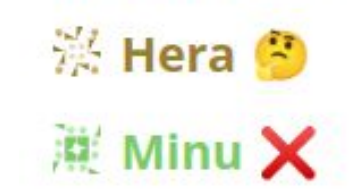
\includegraphics[height=2.5em]{images/nochat.png}};
    \node[illus, anchor=north] () at (-3.3,-.7) {
\includegraphics[height=2.5em]{images/chat.png}};
    
    \node[illus, anchor=north] () at (-3.35,2) {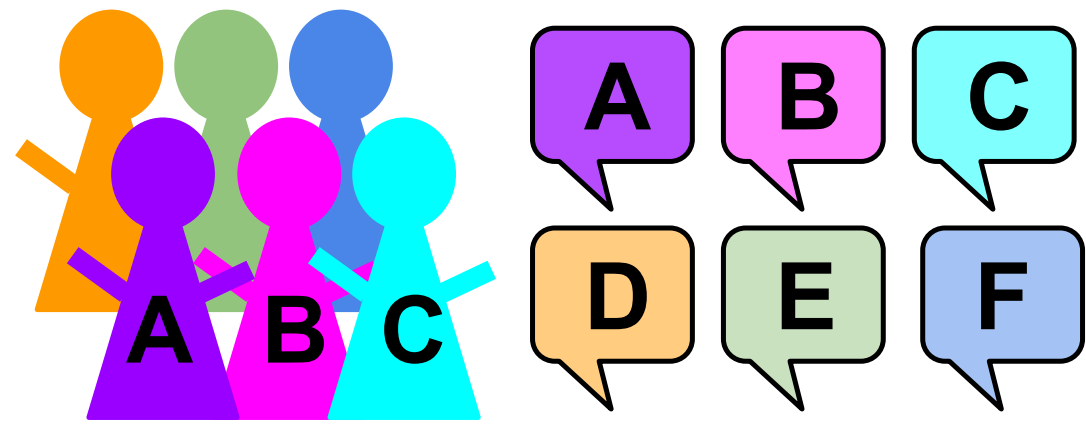
\includegraphics[height=3em]{images/rotate.png}};
    \node[illus, anchor=north] () at (7.5,4.8) {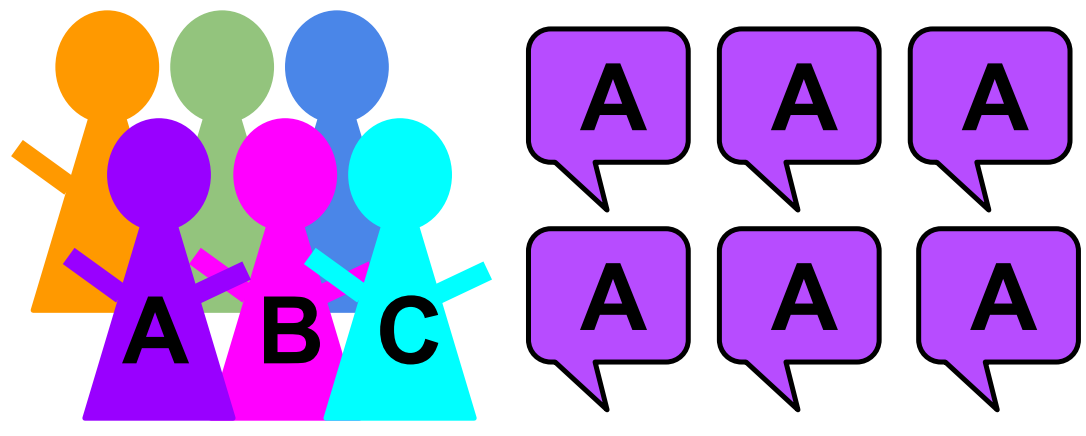
\includegraphics[height=3em]{images/norotate.png}};
    
    
    \node[anchor=north] () at (-1,.7) {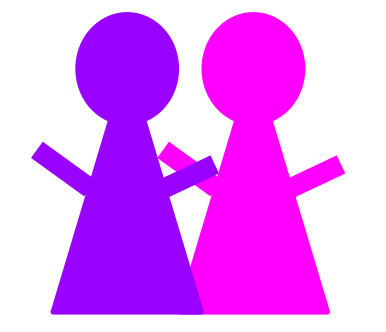
\includegraphics[height=1.5em]{images/two.png}};
    \node[ anchor=north] () at (6.8,.8) {
\includegraphics[height=2em]{images/six.png}};
    
    \node[illus, anchor=north] () at (-4.3,4) { 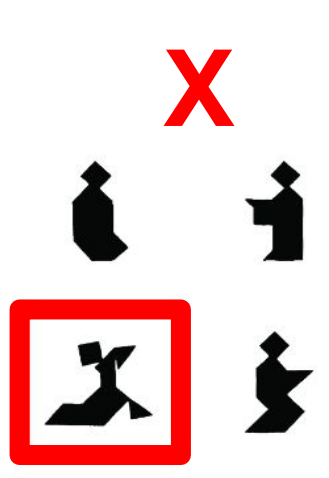
\includegraphics[height=4em]{images/limited-wrong.png}    %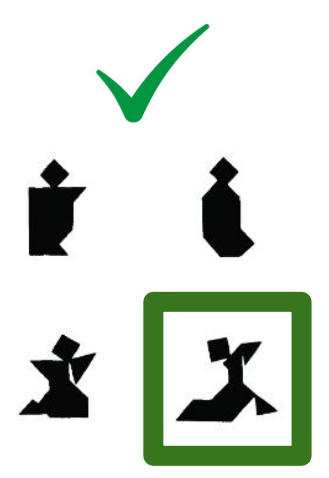
\includegraphics[scale=.1]{images/limited-correct.png}
    };
    \node[illus, anchor=north] () at (8,2.5) {  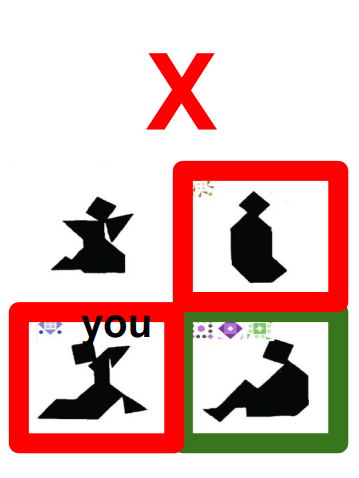
\includegraphics[height=4em]{images/full-wrong.png}   %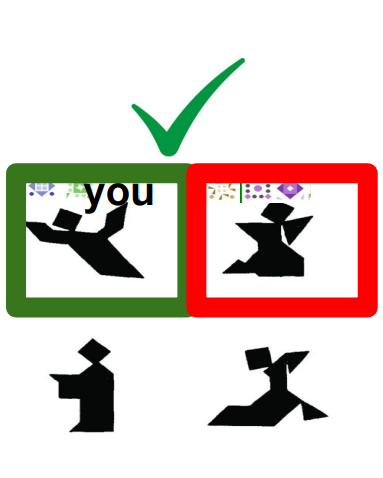
\includegraphics[scale=.1]{images/full-correct.png}
        };
        
        \draw[dashed] (n6) edge [] (n6thin);
        \draw[dashed] (n2thin) edge [] (n6thin);
        \draw[dashed] (n2thick) edge [] (n6thick);
        \draw[dashed] (n6) edge [] (n6thick);
        
        
        \node[illus, anchor=north west] () at (4.75, -1.5) {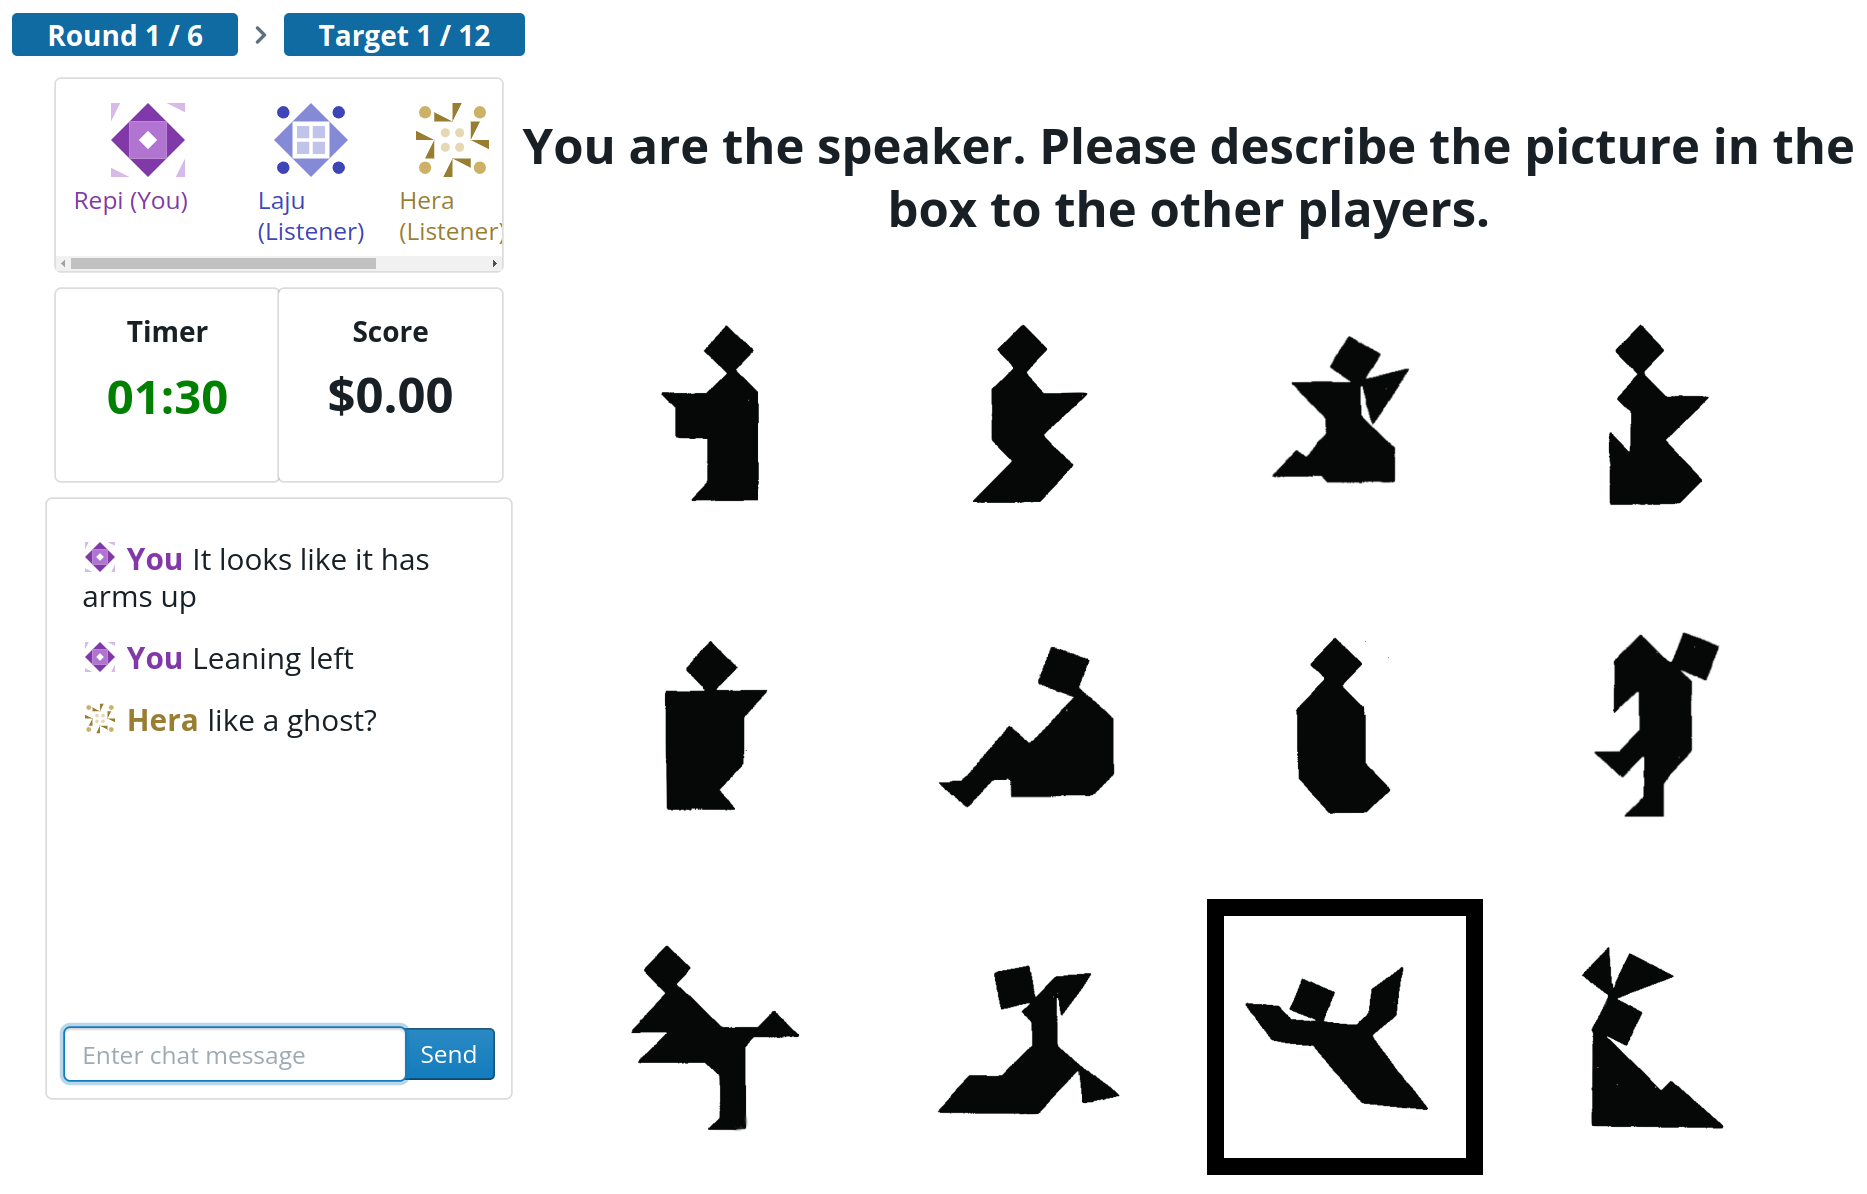
\includegraphics[width=15em]{images/diagram.png}};
        \node[anchor=north west] () at (7, -1) {Trial};
        
        \node[illus, anchor=north west, minimum width=18.5em, minimum height=14.5em] (block) at (4.5, -1) {};
        \node[anchor=north west] () at (7, -.5) {Block};
        \node[anchor=north west] () at (8.5, -5.5) {x 12 images};
        \node[anchor=north west] () at (8.5, -6.1) {x 6 iterations};
        
        \begin{scope}[line width=1 pt, >=Stealth]
            \draw[->] (lab1) -> (n2);
            \draw[->] (lab2) -> (n2thick);
            \draw[->] (lab3) -> (n2);
            \draw[->] (lab4) -> (n2thin);
            
        \end{scope}
        
        
        
    \end{tikzpicture}
    
\caption{ Diagram of the experimental space explored in these experiments. Experiment 1 (pink) has a backchannel where listeners can use the chat and low group coherence from a rotating speaker and limited feedback. Experiment 1's conditions vary the group size from 2 - 6 players. Experiment 2 (blue) games keep group size constant at 6 and vary along the other dimensions. 6 single speaker and 6 full feedback each add one component of group coherence relative to experiment 1. 6 thin varies the backchannel (relative to experiment 1) by having listeners communicate with emoji rather than the full text chat the speaker uses. Experiment 3 (green) tests 4 corners of the space, crossing group size (2 or 6 players) with thin games that have low group coherence and low backchannel or thick games that have high group coherence and high backchannel.  The not-yet-an-inset shows the structure of the experiment, each trial a speaker describes a target image to the listeners, and this process repeats for all 12 images to comprise a block, and the block repeats for a total of 6 iterations. TODO FIX ME AND MY ILLUSTRATION!!! }
    \label{diagram}
\end{figure}

\hypertarget{results}{%
\section{Results}\label{results}}

Across the three experiments and multiple conditions, all iterated reference games shared the same structure amd materials so they are inter-comparable. As shown in Figure \ref{diagram}, all of the games used 12 target images arranged in a grid differently for each player (\protect\hyperlink{ref-clarkReferringCollaborativeProcess1986}{Clark \& Wilkes-Gibbs 1986}, \protect\hyperlink{ref-hawkinsCharacterizingDynamicsLearning2020}{Hawkins et al. 2020}). The speaker knew which image was the target, and their goal was to describe it to their groupmates (listeners) over a chat interface so each listener could select the target. After all listeners had selected, players recieved feedback on the selections. This repeated for all the images with the same speaker to comprise a 12 trial block. Then the whole process repeated for a total of 6 blocks. {[}TODO possibly can reduce this depending on what's in intro{]}.

We extended on the dyadic paradigm of Hawkins et al. (\protect\hyperlink{ref-hawkinsCharacterizingDynamicsLearning2020}{2020}) by parameterizing the experiments along a few dimensions (see Figure \ref{diagram}). One dimension was game size which varied between 2 and 6 player groups; this explores the gradual effects having a larger audience. Another dimension was group coherence, which was made up of two components: speaker rotation and feedback. In low group coherence games, the speaker rotated each block, while in high group coherence games, one player was the speaker for the entire game. Rotating speakers is a more stringent test of convergence because it compares utterances from different players, but having a single speaker gives one person the job of paying attention to what people understand, which could help hold the group together. In low group coherence games, each listener only recieved feedback on if they were indiviually right or wrong in their selection, while in high group coherence games, listeners (like the speakers in all games) saw who had selected what and what the target had been, thus ensuring people saw what referent was intended and had a sense of how everyone else was doing. The last dimension of variation was listener backchannel: in high backchannel games, the listeners could freely send (text) messages to the shared chat, while in the low backchannel games, listeners could send 4 discrete messages (represented as emojis) to the chat. This dimension was inspired by the claimed importance of listener contributions to convention formation {[}TODO CIATIONS{]}

As shown in Figure whatever, Experiment 1 had constant low group coherence and high listener backchannel while varying group size. Experiment 2 held group size constant at 6 and each condition deviated from experiment 1 in one aspect: 6 single speaker and 6 full feedback changed components of group coherence and 6 thin had a low backchannel. Experiment 3 tested 4 corners of the experimental space at larger scale, with thin (low backchannel, low coherence) and thick (high backchannel, high coherence) games with either 2 or 6 players.

We first compare the results on two behavioral measures of listener accuracy and speaker reduction of words that have been the common markers of reduction phenomena in the literature {[}CITE{]}. We then explore semantic patterns of reduction by comparing similarities of utterances to look at how the speaker's language changes within and between games over time.

\hypertarget{behavioral-results}{%
\subsection{Behavioral results}\label{behavioral-results}}

The two key behavioral outcomes were how accurately listeners selected the target images and how many words the speaker produced each trial.

\begin{figure*}[t!]

{\centering \includegraphics[width=1\linewidth]{figs/behavioral-1} 

}

\caption{Behavioral results across all three experiments. A. Listener accuracy at selecting the target image. Dots are per condition, per block estimates with 95\% bootstrapped CIs. Smooths are binomial fit lines. B. Number of words said by the speaker each trial. Faint dots represent individual trials from individual games. Smooths are quadratic fit lines. Y-axis is truncated, and a few outliers points are not visible. }\label{fig:behavioral}
\end{figure*}

Listeners selected the correct target far above chance in every condition, and in every condition, listener accuracy rose over the course of the game (Figure \ref{fig:behavioral}A). Experiment 1 found no strong effects of group size on overall accuracy (numPlayers: -0.07 {[}-0.2, 0.05{]}) or improvement rate (block:numPlayers: -0.02 {[}-0.05, 0.01{]}). In experiment 3, participants in six player games were less accurate (gameSize6: -0.64 {[}-1.05, -0.25{]}) and slower to improve (block:gameSize6: -0.34 {[}-0.43, -0.25{]}) than players in 2 player games, but thin versus thick games did not have a clear effect on accuracy (block:channelthin: -0.07 {[}-0.18, 0.04{]}) or improvement rate (block:channelthin: -0.07 {[}-0.18, 0.04{]}). The high and increasing levels of accuracy indicate that across all of these conditions, participants are able to play the game and succeed in communicating about the images.

The key observation in iterated reference games is that the descriptions the speaker gives of the target images start out long and become shorter over the course of repetitions. This pattern of reduction held across all conditions, with the numbers of words from the speaker decreasing over blocks (Figure \ref{fig:behavioral}B), although there were substantial differences in how verbose speakers were across games. In experiment 1, the overall effect of being one block later was -3.37 {[}-4.54, -2.24{]} words. Speakers in larger groups said more; the effect of each additional player was 1.66 {[}0.66, 2.61{]} words per trial, with no clear interaction between block and group size (block:numPlayers: -0.1 {[}-0.36, 0.17{]}). In experiment 2, the result of being one block later on the number of words the speaker said per trial was block: -5.39 {[}-6.46, -4.31{]} for 6 single speaker; block: -4.68 {[}-5.88, -3.52{]} for 6 full feedback, and block: -2.15 {[}-3.44, -1.12{]} for 6 thin. The rate of reduction was lower in the thin condition than in the other conditions. In experiment 3, reduction occurred overall (block: -2.29 {[}-2.95, -1.6{]}). The six player games said more to start with (gameSize6: 7.41 {[}3.57, 11.18{]}) and reduced less (block:gameSize6: -1.21 {[}-2.06, -0.3{]}) than the two-player games. There were not significant differences due to channel type (channelthin: 0.63 {[}-3.18, 4.73{]}) or channel type over time (block:channelthin: 0.32 {[}-0.65, 1.24{]}).

TODO possibly say more about group to group variation

These reduction results confirm and extend what was previously known for 2 player games. Behaviorally, larger games are similar to smaller games, but their speakers tend to say more overall, perhaps related to the increased number of listeners to respond to.

What about the listeners? Compared to how much referential language speakers produce, listeners produce very little, and it is concentrated in the early rounds. TODO say more about listener language including some numbers!!!

\hypertarget{comparisons-of-language-between-and-within-games}{%
\subsection{Comparisons of language between and within games}\label{comparisons-of-language-between-and-within-games}}

\begin{figure}


        \definecolor{div}{HTML}{006400}
\tikzset{
mynode/.style={
draw, rectangle, align=center,  text width=4cm, scale=1, font=\small, inner sep=.5ex, anchor=north east},
}

\begin{tikzpicture}
\node[mynode] (a0) at (1.5, 9.6) {\textbf{Round 1:} stomping feet, head is not the highest point of the picture - maybe a shoulder is at the same height, both feet point left};
\node[mynode] (a1) at (1.5, 7.1)  {\textbf{Round 2:} diamond head is almost on back and on right side of body; both feet are pointing left
};
\node[mynode] (a2) at (1.5, 5.4)  {\textbf{Round 3: }sad guy with square backpack, feet to the left
};
\node[mynode] (a3) at (1.5, 4.1) { \textbf{Round 4:} stomping feet pointing left; square backpack on right; nose pointing down on left
};
\node[mynode] (a4) at (1.5, 2.4) { \textbf{Round 5:} sad guy with backpack, legs to the left
};
\node[mynode] (a5)  at (1.5,1.4) {\textbf{Round 6:} sad guy with backpack, legs to the left
};

\node[mynode] (b0) at (-3.5,9.6) {\textbf{Round 1:} like someone dancing, with one foot on the ground and one up a little, facing left, like a head yes, like they are kind of leaning back, foot sticking out a little to the left};
\node[mynode] (b1) at (-3.8,6.6)  {\textbf{Round 2:} Like a man facing left marching with a flag over his shoulder, Face is pointy looking down
};
\node[mynode] (b2) at (-4.1,4.7) {\textbf{Round 3:} looking to the left one leg up pointy face
};
\node[mynode] (b3) at (-4.4,3.6) {\textbf{Round 4:} man marching with flag over shoulder
};
\node[mynode] (b4) at (-4.7,2.5)  { \textbf{Round 5:} marching man with flag over shoulder
};
\node[mynode] (b5)   at (-5,1.2) { \textbf{Round 6:} flag bearer};


\node[align=center, color=blue, anchor=north west] at (-10.5,10) {\textbf{Convergence} \\ \textbf{within a game}};
\node[align=center, color=div, anchor= north west] at (-5,10) {\textbf{Divergence between games}}; 

\node[] at (-10,8) {
\includegraphics[width=4em]{images/tangram_A.png}};
    \begin{scope}[line width=1 pt, >=Stealth]
    %\draw [<->]   (a0.west) edge [out=230, in=150] node {.23}  (a5.west);
    %\draw [<->]   (a1.west) edge [out=210, in=150] node [left]{.13} (a5.west);
    %\draw [<->]   (a2.west) edge [bend right] node [left] {.92}(a5.west);
    %\draw [<->]   (a3.west) edge [out=210, in=90] node [left] {.47} (a5.west);
    %\draw [<->]   (a4.south) edge  node [left] {.91} (a5);
    
    \draw [<->, color=blue]   (b0) edge [out=180, in=200] node [inner sep=2ex, left, pos=.1]{.13}  (b5.south west);
    \draw [<->, color=blue]   (b1) edge [out=180, in=200] node [inner sep=3ex, left, pos=.1]{.53}  (b5.west);
    \draw [<->, color=blue]   (b2) edge [out=180, in=150] node  [inner sep=4ex, left, pos=0]{.13}  (b5.west);
    \draw [<->, color=blue]   (b3) edge [out=180, in=150] node [inner sep=3ex, left, pos=0] {.62} (b5.north west);
    \draw [<->, color=blue]   (b4.west) edge [out=270, in=90]node [inner sep=.5ex, left, pos=0]{.63} (b5.north west);
    
    \draw [<->, color=div]   (a0) edge [pos=.5, ".59"] (b0);
    \draw [<->, color=div]   (a1) edge [pos=.8, ".29"] (b1);
    \draw [<->, color=div]   (a2) edge [pos=.8, ".48"] (b2);
    \draw [<->, color=div]   (a3) edge [pos=.5, ".28"] (b3);
    \draw [<->, color=div]   (a4) edge [pos=.5, ".32"] (b4);
    \draw [<->, color=div]   (a5) edge [pos=.5, ".06"] (b5);
    

    
\end{scope}

\end{tikzpicture}
\label{sbert-diagram}
\caption{Example utterances describing the shown tangram figure produced by two 3-player games in Experiment 1. To measure convergence within a game (blue), we measured the cosine similarity between SBERT embeddings of descriptions and the embedding of the round 6 utterance (taken to be the convention). Higher cosine similarity indicates more similar meaning. To measure divergence between games (green), we measured the similarity between utterances from the same round across games.}
\end{figure}

In addition to behavioral measures, we can also look at how the descriptions change over time within and between games. The reduction phenomenon is supposed to be a proxy and correlate of a conventionalization of meaning, to something specific to the pair or group. To quantify this and test the relationships of utterances bewteen and within games, we focus on the speaker's description, concatentating it all together into one utterance (this includes any add ons or answers to questions). Then we use SBERT to embed the utterance in a high-dimensional vector space TODO CITATION. This turns each speaker description into a long vector, where the vectors represent some of the semantic content of the utterance. Vectors that are close together represent utterances that are more similar to one another, so by looking at cosine similarity (a metric of how close pairs of vectors are) we can see how similar pairs of utterances are.

As a measure of convention formation, we can track how utterances describing the same tangram become increasingly similar over the course of a game. If conventions are forming we expect the similarity to the last block utterance to increase over the course of the game.

If different games go in different directions with their descriptions, we'd expect this similarity between descriptions of the same image in different games to decrease over repetitions. Example utterances and their similiarities are illustrated in Figure \ref{sbert-diagram}.

\begin{figure*}[t!]

{\centering \includegraphics[width=1\linewidth]{figs/sbert-1} 

}

\caption{Language similarity results measured with pairwise cosine similarity between embeddings of two utterances. A. Convergence of utterances within games as measured by similarity between an utterance from block 1-5 to the block 6 utterance in the same game for the same image. Dots are per-game averages, smooths are quadratic. B. Divergence of utterances across games as measured by the similarity between an utterances and utterances produced for the same image by different groups in the same block. Dots are per-image averages, smooths are quadratic.}\label{fig:sbert}
\end{figure*}

We first look at convergence, comparing utterances from the first 5 rounds of a game to the ``convention'' or round 6 utterance for the same figure. As visible in Figure \ref{fig:sbert}A, similarity the last utterances occurs across all conditions. In experiment 1, the similarity of the first utterance to last utterances is invariant across group size (-0.01 {[}-0.02, 0{]}), but smaller groups converge faster (-0.01 {[}-0.01, -0.01{]}). Experiment 2 shows similar patterns of utterances become more similar to the last utterance, particularly in the single speaker condition (0.09 {[}0.08, 0.09{]}) where all the utterances come from the same person, but also in the full feedback condition (0.06 {[}0.05, 0.07{]}) and to a smaller extent, in the thin condition (0.02 {[}0.01, 0.03{]}). In experiment 3, convergence is slower in thin games than thick games (-0.02 {[}-0.03, -0.02{]}) and especially thin 6 player games (-0.04 {[}-0.05, -0.02{]}).

Not only do groups reduce the lengths of their utterances, but each group is converging towards a semantic description for the figures. This is more prominent in smaller games and games with greater group coherence.

The complement to convergence within groups is divergence between groups, as different groups develop their own ways of identifying the different figures. In experiment 1, descriptions become less similar to those used to describe the same figure in other games (-0.04 {[}-0.04, -0.03{]}). Group size does not affect the cross-groups similarities in the first block (0 {[}0, 0{]}), but smaller groups diverge from each other faster than larger groups (0 {[}0, 0{]}). In experiment 2, divergence is stronger in the single speaker (-0.04 {[}-0.04, -0.04{]}) and full feedback conditions (-0.04 {[}-0.04, -0.04{]}) than in the 6 thin condition (0 {[}-0.01, 0{]}). In experiment 3, descriptions from different games get less similar over time (-0.02 {[}-0.02, -0.02{]}). There are slight differences in the initial starting points across the different conditions, as well as slight condition differences in how fast the games diverge. In particular, 6 player thin games diverge more slowly (0.02 {[}0.02, 0.02{]}).

TODO possibly say more about 6 thin and check modelling issues

Comparing embeddings of utterances also gives more details. As shown in Appendix figure, the similarity the last utterance can be seen as the cumulative similarities of consecutive utterances. Over time adjacent utterances become more similar as the utterances converge closer to a convention. As group narrow in on descriptions for each image, names for tangrams become more distinctive. While initially, many tangrams might be described in terms of shapes or body parts and directions, as the get nicknames, they differentiate more (See supp figure). All of these confirm expected patterns.

TODO say more about this

\hypertarget{todo-theres-a-note-saying-to-rerun-these-models-for-longer-with-more-extensive-mixed-effects-at-least-of-reduction-model}{%
\subsubsection{TODO there's a note saying to rerun these models for longer with more extensive mixed effects!! (at least of reduction model)}\label{todo-theres-a-note-saying-to-rerun-these-models-for-longer-with-more-extensive-mixed-effects-at-least-of-reduction-model}}

\hypertarget{general-discussion}{%
\section{General Discussion}\label{general-discussion}}

this isn't the only group dynamic; could imagine situations where listeners can see each others work collaborate (point to each other what htey think, perhaps see feedback from speaker to one listener) which might make things reduce much faster

The emergence of conventions has been a key case study for communication more broadly. Yet this issue has -- for the most part -- been studied only in dyadic communication. While some studies have examined aspects of convention formation in larger groups (e.g., \protect\hyperlink{ref-yoonAdjustingConceptualPacts2014}{Yoon \& Brown-Schmidt 2014}, \protect\hyperlink{ref-yoonAudienceDesignMultiparty2019}{Yoon \& Brown‐Schmidt 2019}), basic descriptive work has not yet investigated how group size changes the dynamics of interaction in a standard referential communication task, in part because such tasks can be difficult to administer to larger groups. Taking advantage of a new online multi-player experiment platform, we ran repeated reference games with groups of 2--6 players and characterized the nature of group performance.

Consistent with dyadic games, listeners' selection accuracy increased over blocks at the same time as listeners sped up their selections (question 1).
Crucially, speakers reduced the length of their descriptive utterances as they conventionalized on concepts for each image (question 2). Because speakers rotated, this reduction finding is robust: not only did speakers say less in later repetitions than they themselves said earlier, speakers later in the order said less than speakers earlier in the rotation. This reduction varied with group size; smaller groups used shorter utterances, but group size did not significantly interact with block (question 3). The trajectory of reduction also depended on whether the current speaker correctly identified the tangram in the prior block and whether the current speaker was new to being speaker. This pattern is consistent with both the `aim low' and `aim middle' hypotheses from previous work (\protect\hyperlink{ref-yoonAdjustingConceptualPacts2014}{Yoon \& Brown-Schmidt 2014}, \protect\hyperlink{ref-yoonAudienceDesignMultiparty2019}{Yoon \& Brown‐Schmidt 2019}).

What was specifically different across group sizes? Smaller groups showed more agreement in how each tangram was identified across blocks (question 4), coming to consensus earlier: Their overlap between descriptions in the first 5 blocks to the final block was higher, and words in the final block tended to originate earlier. The greater diversity in how tangrams were described in larger groups could be explained by slower convergence to a convention or parallel competing conceptualizations favored by different speakers. Larger groups have more people for the speaker to communicate to, but also more people who might interrupt with questions, and more people who have opinions about what each image looks like. Bigger groups differ from smaller groups in a number of ways, however, and disentangling these differences is an area for future work.

Group interactions are rich, and this experiment is necessarily a schematic simplification with a number of limitations. Real-life situations vary widely in who the interlocuters are, their relationships, their goals, and their environment (\protect\hyperlink{ref-carletta1998}{Carletta et al. 1998}, \protect\hyperlink{ref-fay2000}{Fay et al. 2000}). Our participants were a convenience sample of Prolific workers who were strangers to each other; thus we miss richness that could come from prior relationships or shared community. Reference is only one goal out of many possible communicative goals, and the tangram images are artificial.
We provided less feedback than previous studies such as Hawkins et al. (\protect\hyperlink{ref-hawkinsCharacterizingDynamicsLearning2020}{2020}); this regime imitates situations where interlocutors can't show each other examples, but it's not representative of all communicative environments. Further, our text-based online paradigm meant that participants' individual identities were not especially salient. In sum, communication takes place in a plethora of situations; our experiment provides some insights, but also misses many complexities that should be a focus of further experiments.

The experimental paradigm presented here could be a valuable tool to disentangle the mechanisms of group size and determine which design parameters are relevant to reduction. Luckily, with an online implementation, recruiting for and running experiments is feasible, and thus it will be possible to iterate on this experiment to determine how far the patterns generalize. While much is left to be explored, this initial data set provides a rich corpus of how humans adapt language dynamically to communicate.

\hypertarget{limitations}{%
\subsection{Limitations}\label{limitations}}

\hypertarget{methods}{%
\section{Methods}\label{methods}}

We extended the dyadic repeated reference game paradigm of Hawkins et al. (\protect\hyperlink{ref-hawkinsCharacterizingDynamicsLearning2020}{2020}) along a few dimensions. As diagrammed in Figure \ref{diagram}, three dimensions of variation we considered were group size, listener backchannel, and group coherence. In experiment 1, we expanded from dyadic reference games to group games with 2--6 players who rotated between speaker and listener roles. In experiment 2, we built on the 6 player games by exploring three variations, two which increased group coherence by increasing feedback to listeners or having a single speaker for the entire game, and one that reduced the listener backchannel. For experiment 3, we considered the extremes of group size and performance, informed by the prior experiments. The thin channel repeated the reduced-backchannel, low-group coherence condition, and we created a thick channel by combining the two sources of group coherence together. We then crossed these thick and thin condition with groups of 2 and 6 players and collected more data in each of these conditions.

For all experiments, we used Empirica (\protect\hyperlink{ref-almaatouqEmpiricaVirtualLab2020}{Almaatouq et al. 2020}) to create real-time multi-player reference games. In each game, one of the players started as the speaker who saw an array of tangrams with one highlighted (Figure \ref{game}A) and communicated which figure to click to the other players (listeners). After the speaker had identified each of the 12 images in turn, the process repeated with the same images, but a total of 6 blocks (72 trials). We recorded what participants said in the chat, as well as who selected what image and how long they took to make their selections.

These experiments were designed sequentially and pre-registered individually.\footnote{Experiment 1: \url{https://osf.io/cn9f4} for the 2-4 player groups, and \url{https://osf.io/rpz67} for the 5-6 player data run later. Experiment 2: single speaker at \url{https://osf.io/f9xyd}, full feedback at \url{https://osf.io/j5zbm}, and thin at \url{https://osf.io/k5f4t}. Experiment 3: \url{https://osf.io/untzy}} TODO more comments on pre-reg

\hypertarget{participants}{%
\subsection{Participants}\label{participants}}

\begin{table}

\caption{\label{tab:participants}The number of games in each experiment and condition. Complete games finished all 6 blocks; partial games ended early due to disconnections, but contributed at least one complete block of data. 6* indicates that some games started with fewer than 6 players or continued with fewer than 6 players after participants disconnected.}
\centering
\begin{tabular}[t]{l|l|r|r|r}
\hline
Experiment & Players & Complete & Partial & Total Participants\\
\hline
1: baseline & 2 & 15 & 4 & 38\\
\hline
1: baseline & 3 & 18 & 2 & 60\\
\hline
1: baseline & 4 & 19 & 2 & 84\\
\hline
1: baseline & 5 & 17 & 3 & 100\\
\hline
1: baseline & 6 & 12 & 6 & 108\\
\hline
2: single speaker & 6 & 15 & 3 & 108\\
\hline
2: full feedback & 6 & 13 & 4 & 102\\
\hline
2: thin & 6 & 10 & 6 & 96\\
\hline
3: thin & 2 & 35 & 3 & 76\\
\hline
3: thin & 6* & 44 & 0 & 235\\
\hline
3: thick & 2 & 39 & 3 & 84\\
\hline
3: thick & 6* & 38 & 2 & 222\\
\hline
\end{tabular}
\end{table}

Participants were recruited using the Prolific platform, and all participants self-reported as fluent native English speakers on Prolific's demographic prescreen. Participants each took part in only one experiment. Experiment 1 took place between May and July 2021, experiment 2 between March and August 2022, and experiment 3 in October 2022. As games varied in length depending on the number of participants, we paid participants based on group size, with the goal of a \$10 hourly rate. Participants were paid \$7 for 2-player games, \$8.50 for 3-player games, \$10 for 4-player games, and \$11 for 5- and 6-player games. When one player had the speaker role for the entirety of a 6-player game, they gained an addition \$2 bonus. Across all games, each participant could early up to \$2.88 in performance bonuses. A total of 1319 people participated across the 3 experiments. A breakdown of number of games and participants in each condition is shown in Table \ref{tab:participants}.

\hypertarget{materials}{%
\subsection{Materials}\label{materials}}

We used the 12 tangram images used by Hawkins et al. (\protect\hyperlink{ref-hawkinsCharacterizingDynamicsLearning2020}{2020}) and Clark \& Wilkes-Gibbs (\protect\hyperlink{ref-clarkReferringCollaborativeProcess1986}{1986}) (see Figure \ref{game}). These images were displayed in a grid with order randomized for each participant (thus descriptions such as ``top left'' were ineffective as the image might be in a different place on the speaker's and listeners' screens). The same images were used every block.

\hypertarget{procedure}{%
\subsection{Procedure}\label{procedure}}

The experimental procedure was very similar across the three experiments. We first describe the procedure used in experiment 1 and then describe the differences in later experiments.

\hypertarget{experiment-1}{%
\subsubsection{Experiment 1}\label{experiment-1}}

We implemented the experiment using Empirica, a Javascript-based platform for running real-time interactive experiments online (\protect\hyperlink{ref-almaatouqEmpiricaVirtualLab2020}{Almaatouq et al. 2020}). From Prolific, participants were directed to our website where they navigated through a self-paced series of instruction pages explaining the game. Participants had to pass a quiz to be able to play the game. They were then directed to a ``waiting room'' screen until their partners were ready.

Once the game started, participants saw screens like Figure \ref{game}A. Each trial, the speaker described the highlighted tangram image so that the listeners could identify and click it. All participants were free to use the chat box to communicate, but listeners could only click once the speaker had sent a message. Once a listener clicked, they could not change their selection. There was no signal to the speaker or other listeners about who had already made a selection.

Once all listeners had selected (or a 3-minute timer ran out), participants were given feedback (Figure \ref{game}B). Listeners learned whether they individually had chosen correctly or not; listeners who were incorrect were not told the correct answer. The speaker saw which tangram each listener had selected, but listeners did not. Listeners got 4 points for each correct answer; the speaker got points equal to the average of the listeners' points. These points translated into performance bonus at the end of the experiment.

In each block, each of the 12 tangrams was indicated to the speaker once. The same person was the speaker for an entire block, but participants rotated roles between blocks. Thus, over the course of the 6 blocks, participants were speakers 3 times in 2-player games, twice in 3-player games, once or twice in 4 and 5-player games, and once in 6-player games. Rotating the speaker was chosen to keep participants more equally engaged (the speaker role is more work), and to give a more robust test for reduction and convention.

After the game finished, participants were given a survey asking for optional demographic information and feedback on their experience with the game.

\hypertarget{differences-in-experiment-2}{%
\subsubsection{Differences in experiment 2}\label{differences-in-experiment-2}}

Experiment 2 consisted of three different variations on Experiment 1, all conducted in 6 player games. Each of these conditions differed from the experiment 1 baseline in one way. The single speaker condition differed only in that one person was designated the speaker for the entire game, rather than having the speaker role rotate. The full feedback condition differed from experiment 1 in that all participants were shown what each person had selected and what the right answer was; listeners still saw text saying whether they individually were right or wrong. This was similar to some dyadic work, such as Hawkins et al. (\protect\hyperlink{ref-hawkinsCharacterizingDynamicsLearning2020}{2020}) where listeners were shown what the right answer was during feedback. For the thin condition, we altered the chatbox interface for listeners. Instead of a textbox, listeners had 4 buttons, each of which sent a different emoji to the chat. Listeners were given suggested meanings for the 4 emojis during instructions. They could send the emojis as often as desired, for instance, initially indicating confusion, and later indicating understanding. In addition, we added notifications that appeared in the chat box saying when a player had made a selection.

\hypertarget{differences-in-experiment-3}{%
\subsubsection{Differences in experiment 3}\label{differences-in-experiment-3}}

The thin channel condition in experiment 3 was the same as the thin condition in experiment 2, above. The thick condition combined the two group coherency enhancing variations from experiment 2: one perspon was the designated speaker throughout, and the feedback participants received included the right answer and what each player had selected. TODO confirm. Across both conditions in experiment 3, notifications were sent to the chat to indicate when a participant had made a selection.

\hypertarget{data-pre-processing-and-exclusions}{%
\subsection{Data pre-processing and exclusions}\label{data-pre-processing-and-exclusions}}

Participants could use the chat box freely, which meant that the chat transcript contained some non-referential language. The first author skimmed through the chat transcripts, tagging utterances that did not refer to the current tangram. These were primarily pleasantries (``Hello''), meta-commentary about how well or fast the task was going, and confirmations or denials (``ok'', ``got it'', ``yes'', ``no''). We exclude these utterances from our analyses. Note that chat lines sometimes included non-referential words in addition to words referring to the tangrams (``ok, so it looks like a zombie'', ``yes, the one with legs''); these lines were retained intact.

In experiments 1 and 2, games did not start if there were not enough participants and ended if any participant disconnected. In experiment 3, games started after a waiting period even if they were not full and continued even after a participant disconnected (with speaker role reassigned if necessary), unless the game would drop below 2 players. The distribution of playes in these 6* player games is at TODO! The realities of online recruitment and disconnection meant that the number of games varied, although we aimed for 20 games in each condition in experiments 1 and 2, and 40 per condition in experiment 3. We excluded incomplete blocks from analyses, but included complete blocks from partial games (See Table \ref{tab:participants} for counts).

When skimming transcripts to tag non-referential utterances, we noticed that one game in the 6-player thick game had a speaker who did not give any sort of coherent descriptions, even with substantial listener prompting. We excluded this game from analyses.

\hypertarget{modelling-strategy}{%
\subsection{Modelling strategy}\label{modelling-strategy}}

TODO
In experiment 3, some of the 6 player games did not have 6 players for the entire game. We do not model this, as it is unclear at what point in the game group size is most relevant. We note that this is a conservative choice that will underestimate differences between 2 player and (genuine) 6 player games, by labelling some smaller groups as 6 player.

We ran all models in brms (CITE) with weakly regularizing priors. We were often unable to fit the full mixed effects structure that we had pre-registered in a reasonable amount of time, so we included what heirarchical effects were reasonable. (All model results and formulae are reported in TODO supplement). Accuracy results used a logistic model, other results use linear models.

\hypertarget{probably-supplemental-figures}{%
\section{Probably supplemental figures}\label{probably-supplemental-figures}}

\begin{figure*}[t!]

{\centering \includegraphics[width=1\linewidth]{figs/listeners-1} 

}

\caption{TODO this probably goes in a supplement! }\label{fig:listeners}
\end{figure*}

\begin{figure*}[t!]

{\centering \includegraphics[width=1\linewidth]{figs/listeners2-1} 

}

\caption{TODO this probably goes in a supplement! }\label{fig:listeners2}
\end{figure*}

\begin{figure*}[t!]

{\centering \includegraphics[width=1\linewidth]{figs/other-1} 

}

\caption{Stuff probably not to include. A is similarity to first utterance. B is similarity between utterances from adjacent blocks. C is divergence in descriptions of different tangrams within a group}\label{fig:other}
\end{figure*}

\hypertarget{distinctiveness-of-tangrams}{%
\subsubsection{Distinctiveness of tangrams}\label{distinctiveness-of-tangrams}}

Another way of looking at how language changes over the course of the game is looking at how games start to refer to different tangrams more differently. This could reflect initial overlap in descriping many figures as sitting or standing or by leg and arm and head position.

Over the course of the game, descriptions for each tangram become more distinctive (-0.04 {[}-0.05, -0.04{]}).
In all three subexperiments, the descriptions of tangrams become more distinctive within games across time. (2a -0.05 {[}-0.05, -0.04{]}, 2b -0.03 {[}-0.03, -0.02{]}, 2c -0.03 {[}-0.03, -0.02{]}).

Tangram distinctiveness within games increased over time (-0.03 {[}-0.03, -0.03{]}). There might be more to say about other effects, but it's mostly a starting places being different in larger games and then the slopes also differ a bit?

\hypertarget{play-with-more-diagrams}{%
\subsubsection{play with more diagrams}\label{play-with-more-diagrams}}

Comparing utterances between adjacent rounds reveals similar patterns. Thin games have lower similarity between adjacent blocks (-0.12 {[}-0.16, -0.09{]}) as do larger games (-0.03 {[}-0.07, 0{]}). Later in the game adjacent blocks are more similar than earlier adjacent blocks (0.05 {[}0.04, 0.05{]}), painting an overall nonlinear convergent pattern (as seen in Figure \ref{fig:other}).

The last measure of how utterances change within games is how they compare to the first utterance; this is less good because the first utterance has more fluffy language so is less diagnostic, but later utterances are further from the first round utterance than earlier utterances (-0.03 {[}-0.04, -0.03{]}). (TODO it's in the pre-reg, but we could dump it in a supplement? )

\hypertarget{supplemental-all-the-models-when-they-were-pre-regd}{%
\section{Supplemental all the models \& when they were pre-reg'd}\label{supplemental-all-the-models-when-they-were-pre-regd}}

\begin{table}

\caption{\label{tab:unnamed-chunk-17}Experiment 1 logistic model of listener accuracy:\\ correct.num $\sim$ block $\times$ numPlayers + (1|gameId)}
\centering
\begin{tabular}[t]{l|l|l}
\hline
Term & Est. & CrI\\
\hline
block & 0.44 & [0.31, 0.58]\\
\hline
block:numPlayers & -0.02 & [-0.05, 0.01]\\
\hline
Intercept & 2.10 & [1.57, 2.65]\\
\hline
numPlayers & -0.07 & [-0.2, 0.05]\\
\hline
\end{tabular}
\end{table}

\hypertarget{references}{%
\section{References}\label{references}}

\setlength{\parindent}{-0.1in} 
\setlength{\leftskip}{0.125in}

\noindent

\hypertarget{refs}{}
\begin{CSLReferences}{1}{0}
\leavevmode\vadjust pre{\hypertarget{ref-almaatouqEmpiricaVirtualLab2020}{}}%
Almaatouq A, Becker J, Houghton JP, Paton N, Watts DJ, Whiting ME (2020) \href{http://arxiv.org/abs/2006.11398}{Empirica: A virtual lab for high-throughput macro-level experiments}. \emph{ArXiv200611398 Cs}

\leavevmode\vadjust pre{\hypertarget{ref-branigan2006}{}}%
Branigan H (2006) Perspectives on multi-party dialogue. \emph{Research on Language and Computation} \textbf{4}:153--177

\leavevmode\vadjust pre{\hypertarget{ref-carletta1998}{}}%
Carletta J, Garrod S, Fraser-Krauss H (1998) Placement of {Authority} and {Communication Patterns} in {Workplace Groups}: {The Consequences} for {Innovation}. \emph{Small Group Research} \textbf{29}:531--559. doi:\href{https://doi.org/10.1177/1046496498295001}{10.1177/1046496498295001}

\leavevmode\vadjust pre{\hypertarget{ref-clarkReferringCollaborativeProcess1986}{}}%
Clark HH, Wilkes-Gibbs D (1986) \href{http://www.speech.kth.se/~edlund/bielefeld/references/clark-and-wilkes-gibbs-1986.pdf}{Referring as a collaborative process}. \emph{Cognition}

\leavevmode\vadjust pre{\hypertarget{ref-fay2000}{}}%
Fay N, Garrod S, Carletta J (2000) Group {Discussion} as {Interactive Dialogue} or as {Serial Monologue}: {The Influence} of {Group Size}. \emph{Psychol Sci} \textbf{11}:481--486. doi:\href{https://doi.org/10.1111/1467-9280.00292}{10.1111/1467-9280.00292}

\leavevmode\vadjust pre{\hypertarget{ref-fox-tree2013}{}}%
Fox Tree JE, Clark NB (2013) Communicative {Effectiveness} of {Written Versus Spoken Feedback}. \emph{Discourse Processes} \textbf{50}:339--359. doi:\href{https://doi.org/10.1080/0163853X.2013.797241}{10.1080/0163853X.2013.797241}

\leavevmode\vadjust pre{\hypertarget{ref-ginzburg2005}{}}%
Ginzburg J, Fernandez R (2005) Action at a distance: The difference between dialogue and multilogue. \emph{Proceedings of DIALOR}:9

\leavevmode\vadjust pre{\hypertarget{ref-haber2019}{}}%
Haber J, Baumgärtner T, Takmaz E, Gelderloos L, Bruni E, Fernández R (2019) The {PhotoBook Dataset}: {Building Common Ground} through {Visually-Grounded Dialogue}. In: \emph{Proc. 57th {Annu}. {Meet}. {Assoc}. {Comput}. {Linguist}.} {Association for Computational Linguistics}, {Florence, Italy}, p 1895--1910. Available from: \url{https://www.aclweb.org/anthology/P19-1184} {[}Last accessed 1 February 2022{]}. doi:\href{https://doi.org/10.18653/v1/P19-1184}{10.18653/v1/P19-1184}

\leavevmode\vadjust pre{\hypertarget{ref-hawkinsCharacterizingDynamicsLearning2020}{}}%
Hawkins RD, Frank MC, Goodman ND (2020) \href{http://arxiv.org/abs/1912.07199}{Characterizing the dynamics of learning in repeated reference games}. \emph{ArXiv191207199 Cs}

\leavevmode\vadjust pre{\hypertarget{ref-horton2002}{}}%
Horton WS, Gerrig RJ (2002) {SpeakersÕ} experiences and audience design: Knowing when and knowing how to adjust utterances to addresseesq. \emph{Journal of Memory and Language}:18

\leavevmode\vadjust pre{\hypertarget{ref-horton2005}{}}%
Horton WS, Gerrig RJ (2005) The impact of memory demands on audience design during language production. \emph{Cognition} \textbf{96}:127--142. doi:\href{https://doi.org/10.1016/j.cognition.2004.07.001}{10.1016/j.cognition.2004.07.001}

\leavevmode\vadjust pre{\hypertarget{ref-kraussChangesReferencePhrases1964}{}}%
Krauss RM, Weinheimer S (1964) Changes in reference phrases as a function of frequency of usage in social interaction: A preliminary study. \emph{Psychon Sci} \textbf{1}:113--114. doi:\href{https://doi.org/10.3758/BF03342817}{10.3758/BF03342817}

\leavevmode\vadjust pre{\hypertarget{ref-kraussConcurrentFeedbackConfirmation1966}{}}%
Krauss RM, Weinheimer S (1966) Concurrent feedback, confirmation, and the encoding of referents in verbal communication. \emph{Journal of Personality and Social Psychology} \textbf{4}:343--346. doi:\href{https://doi.org/10.1037/h0023705}{10.1037/h0023705}

\leavevmode\vadjust pre{\hypertarget{ref-schober1989}{}}%
Schober MF, Clark HH (1989) Understanding by addressees and overhearers. \emph{Cognitive Psychology} \textbf{21}:211--232. doi:\href{https://doi.org/10.1016/0010-0285(89)90008-X}{10.1016/0010-0285(89)90008-X}

\leavevmode\vadjust pre{\hypertarget{ref-tolins2016}{}}%
Tolins J, Fox Tree JE (2016) Overhearers {Use Addressee Backchannels} in {Dialog Comprehension}. \emph{Cogn Sci} \textbf{40}:1412--1434. doi:\href{https://doi.org/10.1111/cogs.12278}{10.1111/cogs.12278}

\leavevmode\vadjust pre{\hypertarget{ref-traum2004}{}}%
Traum D (2004) Issues in {Multiparty Dialogues}. In: Dignum F (ed) \emph{Advances in {Agent Communication}}. {Springer Berlin Heidelberg}, {Berlin, Heidelberg}, p 201--211. Available from: \url{http://link.springer.com/10.1007/978-3-540-24608-4_12} {[}Last accessed 1 February 2022{]}. doi:\href{https://doi.org/10.1007/978-3-540-24608-4_12}{10.1007/978-3-540-24608-4\_12}

\leavevmode\vadjust pre{\hypertarget{ref-yoonAdjustingConceptualPacts2014}{}}%
Yoon SO, Brown-Schmidt S (2014) Adjusting conceptual pacts in three-party conversation. \emph{Journal of Experimental Psychology: Learning, Memory, and Cognition} \textbf{40}:919--937. doi:\href{https://doi.org/10.1037/a0036161}{10.1037/a0036161}

\leavevmode\vadjust pre{\hypertarget{ref-yoonAudienceDesignMultiparty2019}{}}%
Yoon SO, Brown‐Schmidt S (2019) Audience {Design} in {Multiparty Conversation}. \emph{Cogn Sci} \textbf{43}:e12774. doi:\href{https://doi.org/10.1111/cogs.12774}{10.1111/cogs.12774}

\end{CSLReferences}


\end{document}
